\section{Results}

\begin{frame}{Controller comparison}

    Different reference signals have been used to evaluate the controllers' performance, including:

    \begin{itemize}
        \item \textbf{Multistep (stars and up \& down)}: a sequence of equally spaced step inputs ($1[mm]$ or $2[mm]$ in amplitude) to assess the controller's response to abrupt set-point changes and its steady-state performance across various set-points.
        \item \textbf{Sinusoidal (discrete)}: a sinusoidal shape (period $2[s]$, amplitude $2[mm]$), but represented as a sequence of discrete steps, to evaluate the controllers' performance in tracking a periodic signal.
    \end{itemize}

    \vspace{9pt}

    All the results here presented are obtained using a Kalman filter to estimate and/or filter the system's state.

\end{frame}



\begin{frame}{Controller comparison}

    \vspace{9pt}

    \begin{figure}[H]
        \centering
        \includegraphics[width=1\linewidth]{./img/MATLAB/results/multisteps_stairs_star_KF.pdf}
        \caption{Comparison of controllers with multistep stairs reference using KF}
    \end{figure}

\end{frame}



\begin{frame}{Controller comparison}

    \vspace{9pt}

    \begin{figure}[H]
        \centering
        \includegraphics[width=1\linewidth]{./img/MATLAB/results/multisteps_updown_star_KF.pdf}
        \caption{Comparison of controllers with multistep up \& down reference using KF}
    \end{figure}

\end{frame}



\begin{frame}{Controller comparison}

    \vspace{9pt}

    \begin{figure}[H]
        \centering
        \onslide<1->{\includegraphics[width=0.32\linewidth]{./img/MATLAB/results/multisteps_up_PIDstar_KF.pdf}}
        \hfill
        \onslide<2->{\includegraphics[width=0.32\linewidth]{./img/MATLAB/results/multisteps_up_LQstar_KF.pdf}}
        \hfill
        \onslide<3->{\includegraphics[width=0.32\linewidth]{./img/MATLAB/results/multisteps_up_MPCstar_KF.pdf}}
        \caption{PIDs, LQs, MPC with multistep up reference using KF}
    \end{figure}

\end{frame}



\begin{frame}{Controller comparison}

    \vspace{9pt}

    \begin{figure}[H]
        \centering
        \onslide<1->{\includegraphics[width=0.32\linewidth]{./img/MATLAB/results/multisteps_down_PIDstar_KF.pdf}}
        \hfill
        \onslide<2->{\includegraphics[width=0.32\linewidth]{./img/MATLAB/results/multisteps_down_LQstar_KF.pdf}}
        \hfill
        \onslide<3->{\includegraphics[width=0.32\linewidth]{./img/MATLAB/results/multisteps_down_MPCstar_KF.pdf}}
        \caption{PIDs, LQs, MPC with multistep up \& down (down) reference using KF}
    \end{figure}

\end{frame}



\begin{frame}{Controller comparison}

    \vspace{9pt}

    \begin{figure}[H]
        \centering
        \includegraphics[width=1\linewidth]{./img/MATLAB/results/sinusoidal_fast_star_KF.pdf}
        \caption{Comparison of controllers with sinusoidal slow reference using KF}
    \end{figure}

\end{frame}



\begin{frame}{Controller comparison}

    \vspace{9pt}

    \begin{figure}[H]
        \centering
        \onslide<1->{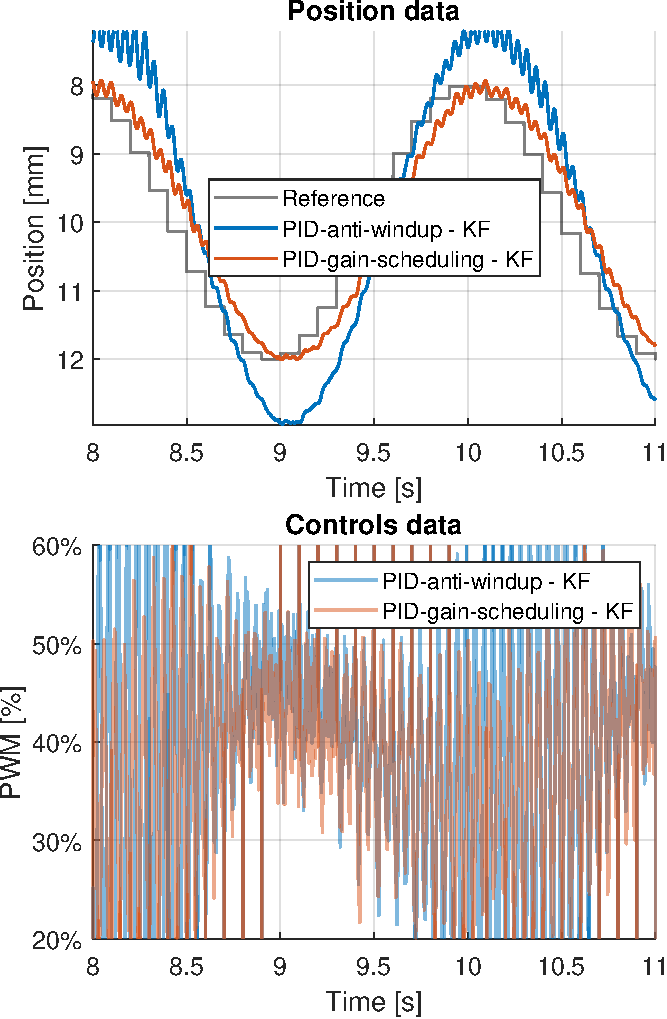
\includegraphics[width=0.32\linewidth]{./img/MATLAB/results/sinusoidal_fast_PIDstar_KF.pdf}}
        \hfill
        \onslide<2->{\includegraphics[width=0.32\linewidth]{./img/MATLAB/results/sinusoidal_fast_LQstar_KF.pdf}}
        \hfill
        \onslide<3->{\includegraphics[width=0.32\linewidth]{./img/MATLAB/results/sinusoidal_fast_MPCstar_KF.pdf}}
        \caption{PIDs, LQs, MPC with sinusoidal fast reference using KF}
    \end{figure}

\end{frame}



\begin{frame}{Controller considerations}

    Overall, from the results obtained, we can draw the following considerations:

    \begin{table}[H]
        \centering
        \renewcommand{\arraystretch}{1}
        \begin{tabular}{|l|c|c|c|c|l|}
            \hline
            \textbf{Controller}          & \textbf{Reactivity} & \textbf{Precision}  & \textbf{Stability} & \textbf{Control} \\ \hline
            \textbf{PID Anti-windup}     & Slow                & Good (steady-state) & Moderate           & High noise       \\ \hline
            \textbf{PID Gain Scheduling} & Good                & Good                & Good               & High noise       \\ \hline
            \textbf{LQR Tracking}        & Very high           & High                & Good               & High noise       \\ \hline
            \textbf{LQI}                 & Very high           & Excellent           & Excellent          & High noise       \\ \hline
            \textbf{MPC}                 & High                & Good                & Good               & Excellent        \\ \hline
        \end{tabular}
        \caption{Controller Comparison}
    \end{table}


\end{frame}


\begin{frame}{Filter \& Estimator comparison}

    To compare filters and estimators, an LQR tracking was used as a controller and a continuous sinusoidal reference signal with a period of $2[s]$ and amplitude of $2[mm]$ was used as a reference signal.

    \vspace{9pt}

    Regarding the estimators, only position and current measurements were used as input, while velocity was estimated.

\end{frame}


\begin{frame}{Filter \& Estimator comparison}

    \vspace{9pt}

    \begin{figure}[H]
        \centering
        \includegraphics[width=1\linewidth]{./img/MATLAB/results/sinusoidal_slow_linear_star_star.pdf}
        \caption{Comparison of filter using an LQR tracking with sinusoidal slow reference}
    \end{figure}

\end{frame}

\begin{frame}{Filter \& Estimator comparison}

    \vspace{9pt}

    \begin{figure}[H]
        \centering
        \includegraphics[width=1\linewidth]{./img/MATLAB/results/sinusoidal_slow_linear_star_star_without_nofilter.pdf}
        \caption{Comparison of filter using an LQR tracking with sinusoidal slow reference}
    \end{figure}

\end{frame}



\begin{frame}{Filter \& Estimator comparison}

    \vspace{9pt}

    \begin{figure}[H]
        \centering
        \includegraphics[width=1\linewidth]{./img/MATLAB/results/sinusoidal_slow_linear_star_star_zoomed_KF_EKF_lowpass.pdf}
        \caption{Comparison of no filter, low pass, KF using an LQR tracking with sinusoidal slow reference}
    \end{figure}

\end{frame}



\begin{frame}{Filter \& Estimator considerations}

    Overall, from the results obtained, we can draw the following considerations:

    \begin{table}[H]
        \centering

        \begin{tabular}{|l|c|c|c|}
            \hline
            \textbf{Filter/Estimator}       & \textbf{Noise reduction} & \textbf{Estimation accuracy} & \textbf{Delay} \\ \hline
            \textbf{No filter}              & -                        & -                            & Absent         \\ \hline
            \textbf{Low-pass filter}        & Good                     & -                            & Minimal        \\ \hline
            \textbf{Luenberg Observer}      & Optimal                  & Extremely inaccurate         & Absent         \\ \hline
            \textbf{Kalman filter}          & Optimal                  & Good                         & Absent         \\ \hline
            \textbf{Extended Kalman filter} & Optimal                  & Inaccurate                   & Absent         \\ \hline
        \end{tabular}
        \caption{Filters and Estimators comparison}
    \end{table}

    \vspace{9pt}

    These results highlight the need for further fine-tuning of the \textbf{EKF}.

\end{frame}